%%
%% This is file `sample-sigconf.tex',
%% generated with the docstrip utility.
%%
%% The original source files were:
%%
%% samples.dtx  (with options: `sigconf')
%% 
%% IMPORTANT NOTICE:
%% 
%% For the copyright see the source file.
%% 
%% Any modified versions of this file must be renamed
%% with new filenames distinct from sample-sigconf.tex.
%% 
%% For distribution of the original source see the terms
%% for copying and modification in the file samples.dtx.
%% 
%% This generated file may be distributed as long as the
%% original source files, as listed above, are part of the
%% same distribution. (The sources need not necessarily be
%% in the same archive or directory.)
%%
%%
%% Commands for TeXCount
%TC:macro \cite [option:text,text]
%TC:macro \citep [option:text,text]
%TC:macro \citet [option:text,text]
%TC:envir table 0 1
%TC:envir table* 0 1
%TC:envir tabular [ignore] word
%TC:envir displaymath 0 word
%TC:envir math 0 word
%TC:envir comment 0 0
%%
%%
%% The first command in your LaTeX source must be the \documentclass command.
\documentclass[compsoc, conference, a4paper, 10pt, times]{IEEEtran}

% Uncomment to enable anonymous submission
%\newcommand*{\ANON}{}%
% Uncomment to make the paper "submission-ready"
\newcommand*{\SUBMISSION}{}%
% Uncomment to make the paper "camera-ready"
\newcommand*{\CAMERAREADY}{}

\newcommand{\clouddate}{2024-03-26}

\newcommand{\sev}{\ac{SEV}}
\newcommand{\seves}{\ac{SEV}-\ac{ES}}
\newcommand{\sevsnp}{\ac{SEV}-\ac{SNP}}
\newcommand{\snp}{\ac{SNP}}
\newcommand{\snpguest}{\texttt{snpguest}}
\newcommand{\sevsnpmeasure}{\texttt{sev-snp-measure}}
\newcommand{\dmintegrity}{\texttt{dm-integrity}}
\newcommand{\dmverity}{\texttt{dm-verity}}
\newcommand{\dmcrypt}{\texttt{dm-crypt}}
\newcommand{\init}{\texttt{/init}}
\newcommand{\vtpm}{\ac{vTPM}}
\newcommand{\sevguest}{\texttt{/dev/sev-guest}}

\ifdefined\SUBMISSION
\usepackage[disable]{todonotes}
\else
\usepackage[textsize=footnotesize]{todonotes}
\presetkeys{todonotes}{fancyline}{}
\setlength{\marginparwidth}{1.3cm}
\setlength{\marginparsep}{3pt}
\fi

\newcommand{\christoph}[1]{\todo[color=orange!20]{\textbf{Christoph:} #1}}
\newcommand{\fritz}[1]{\todo[color=blue!20]{\textbf{Fritz:} #1}}
\newcommand{\gianluca}[1]{\todo[color=red!20]{\textbf{Gianluca:} #1}}
\newcommand{\jt}[1]{\todo{\textbf{JT:} #1}}
\newcommand{\temptext}[1]{\textcolor{blue}{/* #1 */}}

\usepackage{acronym}
\usepackage{enumerate}
\usepackage{subcaption}
\usepackage{pgfplots}
\pgfplotsset{
    width=5cm, 
    legend style={
        font=\footnotesize,
        %rounded corners=2pt
    },
    compat=newest
}
\usepackage[utf8]{inputenc}
\DeclareUnicodeCharacter{2212}{−}
\usepgfplotslibrary{groupplots,dateplot}
\usetikzlibrary{patterns,shapes.arrows}
% timeline diagram
\usetikzlibrary{decorations.pathreplacing,calligraphy}

%\usepackage[cmex10]{amsmath} // TODO this clashes with url and tabularx
\usepackage{url}
\usepackage{tabularx}
\usepackage{fontawesome}
\usepackage{booktabs}
\usepackage{xspace}
\usepackage[pdftex]{hyperref}

%\titleformat{\paragraph}[runin]
%{\bfseries}{\theparagraph}{1em}{}

\newtheorem{req}{Requirement}
\newtheorem{defn}{Definition}
\newtheorem{prop}{Property}

\usepackage[capitalize]{cleveref}
\crefname{figure}{Fig.\@}{Figs.\@}
\Crefname{figure}{Fig.\@}{Figs.\@}
\crefname{table}{Tab.\@}{Tabs.\@}
\Crefname{table}{Tab.\@}{Tabs.\@}
\crefname{section}{Sect.\@}{Sects.\@}
\Crefname{section}{Sect.\@}{Sects.\@}
\crefname{req}{Req.\@}{Reqs.\@}
\Crefname{req}{Req.\@}{Reqs.\@}

\usepackage{paralist}
\usepackage{crossreftools}

\usepackage{fix-cm} % not needed if not using Computer Modern

\DeclareMathAlphabet{\mathsfit}{T1}{\sfdefault}{\mddefault}{\sldefault}
\SetMathAlphabet{\mathsfit}{bold}{T1}{\sfdefault}{\bfdefault}{\sldefault}

\usepackage{listings}

\lstdefinestyle{mystyle}{
    inputpath=listings,
    commentstyle=\color{teal},
    keywordstyle=\color{magenta},
    numberstyle=\tiny\color{gray},
    stringstyle=\color{purple},
    basicstyle=\ttfamily\scriptsize,
    breakatwhitespace=false,         
    breaklines=true,                 
    captionpos=b,                    
    keepspaces=true,                 
    numbers=none,                    
    numbersep=5pt,                  
    showspaces=false,                
    showstringspaces=false,
    showtabs=false,                  
    tabsize=2
}

\lstset{style=mystyle}

\usepackage{balance}


\acrodef{CC}{Confidential Computing}
\acrodef{CCA}{Confidential Compute Architecture}
\acrodef{CEK}{Chip Endorsement Key}
\acrodef{CRL}{Certificate Revocation List}
\acrodef{CSP}{Cloud Service Provider}
\acrodef{CVM}{Confidential Virtual Machine}
\acrodef{AWS}{Amazon Web Services}
\acrodef{ES}{Encrypted State}
\acrodef{GCP}{Google Cloud Platform}
\acrodef{IMA}{Integrity Measurements Architecture}
\acrodef{MitM}{Man-in-the-Middle}
\acrodef{OVMF}{Open Virtual Machine Firmware}
\acrodef{RoTM}{Root of Trust for Measurement}
\acrodef{RTMR}{Runtime Measurement Register}
\acrodef{SEV}{Secure Encrypted Virtualization}
\acrodef{SGX}{Security Guard Extensions}
\acrodef{SNP}{Secure Nested Paging}
\acrodef{SP}{Secure Processor}
\acrodef{SVSM}{Secure VM Service Module}
\acrodef{TCB}{Trusted Computing Base}
\acrodef{TDX}{Trust Domain Extensions}
\acrodef{TEE}{Trusted Execution Environment}
\acrodef{TPM}{Trusted Platform Module}
\acrodef{VMPL}{Virtual Machine Privilege Level}
\acrodef{vTPM}{virtual TPM}


%%
%% Submission ID.
%% Use this when submitting an article to a sponsored event. You'll
%% receive a unique submission ID from the organizers
%% of the event, and this ID should be used as the parameter to this command.
%%\acmSubmissionID{123-A56-BU3}

%%
%% For managing citations, it is recommended to use bibliography
%% files in BibTeX format.
%%
%% You can then either use BibTeX with the ACM-Reference-Format style,
%% or BibLaTeX with the acmnumeric or acmauthoryear sytles, that include
%% support for advanced citation of software artefact from the
%% biblatex-software package, also separately available on CTAN.
%%
%% Look at the sample-*-biblatex.tex files for templates showcasing
%% the biblatex styles.
%%

%%
%% The majority of ACM publications use numbered citations and
%% references.  The command \citestyle{authoryear} switches to the
%% "author year" style.
%%
%% If you are preparing content for an event
%% sponsored by ACM SIGGRAPH, you must use the "author year" style of
%% citations and references.
%% Uncommenting
%% the next command will enable that style.
%%\citestyle{acmauthoryear}


%%
%% end of the preamble, start of the body of the document source.
\begin{document}

%%
%% The "title" command has an optional parameter,
%% allowing the author to define a "short title" to be used in page headers.
%\title{Understanding Trust Relationships in\\Confidential Computing Services in the Cloud}
\title{Understanding Trust Relationships in Cloud-Based Confidential Computing}


%%
%% The "author" command and its associated commands are used to define
%% the authors and their affiliations.
%% Of note is the shared affiliation of the first two authors, and the
%% "authornote" and "authornotemark" commands
%% used to denote shared contribution to the research.
% \author{Gianluca Scopelliti}
% \authornote{Both authors contributed equally to this research.}
% \email{trovato@corporation.com}
% \orcid{1234-5678-9012}
% \author{G.K.M. Tobin}
% \authornotemark[1]
% \email{webmaster@marysville-ohio.com}
% \affiliation{%
%   \institution{Institute for Clarity in Documentation}
%   \streetaddress{P.O. Box 1212}
%   \city{Dublin}
%   \state{Ohio}
%   \country{USA}
%   \postcode{43017-6221}
% }


\newcommand{\affiliationkul}{
  \affiliation{
  \department{DistriNet, KU Leuven, Belgium}
  \institution{}
%   \city{Leuven}
  \country{}
%   \postcode{3001}
  }
}
\newcommand{\affiliationeab}{
  \affiliation{
  \department{Ericsson Security Research, Sweden}
  \city{}
  \country{}
  }
}
\newcommand{\affiliationulb}{
  \affiliation{
%  \department{Ecole Polytechnique, BEAMS \& Cybersecurity Research Center, Universit\'e Libre de Bruxelles, Belgium}
  \department{Universit\'e Libre de Bruxelles, Belgium}
%   \institution{}
%   \city{}
  \country{}
%   \postcode{1050}
  }
}


\ifdefined\ANON
\author{\em Anonymous Author(s)}
\else

\ifdefined\CAMERAREADY
\makeatletter
\newcommand{\linebreakand}{%
  \end{@IEEEauthorhalign}
  \hfill\mbox{}\par
  \mbox{}\hfill\begin{@IEEEauthorhalign}
}
\makeatother

\author{\IEEEauthorblockN{Gianluca Scopelliti}
\IEEEauthorblockA{\textit{Ericsson Security Research, Sweden} \\
%Kista, Sweden \\
\textit{KU Leuven, Belgium} \\
%Leuven, Belgium \\
gianluca.scopelliti@ericsson.com}
\and
\IEEEauthorblockN{Christoph Baumann}
\IEEEauthorblockA{\textit{Ericsson Security Research, Sweden} \\
%Kista, Sweden \\
christoph.baumann@ericsson.com}
\and
\IEEEauthorblockN{Jan Tobias M\"{u}hlberg}
\IEEEauthorblockA{\textit{Universit\'e Libre de Bruxelles, Belgium} \\
%Brussels, Belgium \\
jan.tobias.muehlberg@ulb.be}
}
\else
\author{\IEEEauthorblockN{Gianluca Scopelliti$^{*\dagger{}}$, Christoph Baumann$^{*}$, Jan Tobias M\"{u}hlberg$^{\ddagger{}\dagger{}}$}
\IEEEauthorblockA{
  \textit{$^{*}$Ericsson Security Research, Sweden;
          $^{\dagger{}}$DistriNet, KU Leuven, Belgium;
          $^{\ddagger{}}$Universit\'e Libre de Bruxelles, Belgium} \\
  \textit{gianluca.scopelliti@ericsson.com}
}
}
\fi

\fi

%%
%% By default, the full list of authors will be used in the page
%% headers. Often, this list is too long, and will overlap
%% other information printed in the page headers. This command allows
%% the author to define a more concise list
%% of authors' names for this purpose.
% \renewcommand{\shortauthors}{Anonymous}

%%
%% The code below is generated by the tool at http://dl.acm.org/ccs.cfm.
%% Please copy and paste the code instead of the example below.
%%
%\begin{CCSXML}
%	<ccs2012>
%	   <concept>
%		   <concept_id>10002978.10003006.10003007</concept_id>
%		   <concept_desc>Security and privacy~Operating systems security</concept_desc>
%		   <concept_significance>300</concept_significance>
%		   </concept>
%	   <concept>
%		   <concept_id>10002978.10003006.10003007.10003009</concept_id>
%		   <concept_desc>Security and privacy~Trusted computing</concept_desc>
%		   <concept_significance>500</concept_significance>
%		   </concept>
%	   <concept>
%		   <concept_id>10002978.10003022.10003023</concept_id>
%		   <concept_desc>Security and privacy~Software security engineering</concept_desc>
%		   <concept_significance>300</concept_significance>
%		   </concept>
%	   <concept>
%		   <concept_id>10003033.10003039.10003053.10003054</concept_id>
%		   <concept_desc>Networks~Time synchronization protocols</concept_desc>
%		   <concept_significance>100</concept_significance>
%		   </concept>
%	 </ccs2012>
%	\end{CCSXML}
%	
%	\ccsdesc[300]{Security and privacy~Operating systems security}
%	\ccsdesc[500]{Security and privacy~Trusted computing}
%	\ccsdesc[300]{Security and privacy~Software security engineering}
%	\ccsdesc[100]{Networks~Time synchronization protocols}

%%
%% Keywords. The author(s) should pick words that accurately describe
%% the work being presented. Separate the keywords with commas.
%\keywords{trusted computing, time}
%% A "teaser" image appears between the author and affiliation
%% information and the body of the document, and typically spans the
%% page.

%%
%% This command processes the author and affiliation and title
%% information and builds the first part of the formatted document.
\maketitle

%%
%% The abstract is a short summary of the work to be presented in the
%% article.
\begin{abstract}
  %\boldmath
  A major drawback of cloud computing used to be the lack of confidentiality and
verifiability of computations, making it impossible to use public commercial
clouds to work with sensitive code or data. With the availability of Trusted
Execution Environments (TEEs) came the promise of enabling confidential
computations in the cloud. A number of big Cloud Service Providers (CSP) now
supports the deployment of Confidential Virtual Machines (CVMs) that can be
attested remotely, supposedly guaranteeing verifiable isolation and integrity,
and removing potentially compromised or malicious infrastructure from the
system's Trusted Computing Base (TCB). In this paper, we investigate this claim
and examine the CVM infrastructure provided by commercial CSPs regarding the
attestability of the TEE hardware and the entire CVM software stack, and
transparency regarding software provisioned by the CSP. We develop a hierarchy
of attestation levels to explain our findings and trust limitations. For the
services analysed, we observe that many attestation steps can only partially be
verified by the CVM owner. Thus, running CVMs on these CSPs' infrastructures
does not allow full TCB reduction through independently verifiable attestation
but requires trust in the CSP to deploy secure software and to truthfully report
attestation data. Complete protection from infrastructural threats is thus not
provided.

\end{abstract}

\section{Introduction}
%
Cloud computing is the backbone of digitalized societies, supporting today's
cloud-native web service development paradigm. Increasingly, also industries
that traditionally operated their own IT environments, e.g., telecommunication,
manufacturing, and healthcare, are now moving to the cloud for better
scalability, manageability, and cost reduction. However, this trend is
accompanied by questions about the security and trustworthiness of
\emph{\acp{CSP}} along with regulatory concerns about privacy, data protection,
and data sovereignty: ``moving to the cloud'' involves moving large amounts of
sensitive data, along with some of the responsibility to protect it, to a third
party.

Different forms of \emph{\ac{CC}} have surfaced to address such concerns,
with \emph{\acp{TEE}}~\cite{schneider2022hardware} such as Intel SGX and
TDX, AMD SEV-SNP, or ARM CCA promising to effectively take the cloud
provider out of the \emph{\ac{TCB}}. These \acp{TEE} provide secure
compartments on cloud servers that can run applications while protecting
data in use from infrastructural threats and enabling the ``removal of even
the cloud provider from the Trusted Computing
Base''~\cite{confcon2022marketing}. At the same time they provide
\emph{attestation} mechanisms to cryptographically verify that the
unmodified application is indeed running in an authentic \ac{TEE}.  On
paper, such a design allows for a drastic reduction of customers'
dependency on cloud providers to adequately secure the cloud platform
infrastructure -- firmware, OS, and virtualization layers -- and leaving
only the hardware vendor that implements a \ac{TEE} as a root of trust.

While early \acp{TEE} for server systems embedded \emph{enclaves} into user
processes, the current market trend are \emph{\acp{CVM}} that place an entire
tenant VM into a \ac{TEE}.  While this approach increases the \ac{TCB} within
the \ac{TEE}, it simplifies the deployment of software in \acp{TEE} and reduces
system-call performance overheads~\cite{akram2020performance} relative to
enclaves, thus lowering the \ac{CC} adoption hurdle for customers. Consequently,
cloud providers such as \ac{AWS}, Microsoft Azure, or \ac{GCP} have recently
started marketing \ac{CVM} solutions as an easy fix for the security, privacy,
and trustworthiness challenges outlined above.

However, launching and attesting a \ac{CVM} is a different beast than the
enclave-based \ac{CC} approach. A VM consists of layers of system software,
including firmware, bootloader, kernel, and guest OS, as well as user space
applications, with many components usually provided by the \ac{CSP}.
%% All of these layers, which are provided by the CSP and other
%% software vendors, need to be trusted, measured, and attested during the boot
%% process of the \ac{CVM}.
%% Moreover, a \ac{CVM} needs to be integrated into the cloud platform it is
%% running on, requiring the configuration of storage and networking, but also
%% additional components for monitoring by the cloud provider.
%
Given this large software stack running inside the \ac{CVM}, the issue of
trustworthiness comes again into focus. Effectively removing the infrastructure,
i.e., the \ac{CSP}, from the customer's \ac{TCB} requires
\begin{inparaenum}
\item an attestation infrastructure that allows to attest the authenticity of
  both the \ac{TEE} hardware and \emph{all} the software running inside it, and
\item transparency for software components provisioned by the \ac{CSP} in the
  \ac{CVM}, e.g., by supplying the underlying source code alongside a
  reproducible build process.
\end{inparaenum}

In this paper we examine \ac{CVM} offerings on public clouds along these two
axes in order to evaluate the level of trust in the \ac{CSP} these \ac{CC}
solutions still require.  In particular, we take a close look at the boot
process and provided attestion mechanisms involved in the setup of AMD SEV-SNP
\acp{CVM} on popular cloud providers. It turns out that there are shortcomings
that prevent achieving confidential computing under infrastructural threats. In
many cases this is due to missing attestation infrastructure or proprietary
software components that need to be included in the \ac{CVM}.
% , but a more
% thorough discussion of issues and potential solutions will be given below.
We make the following contributions:
%
\begin{itemize}
%
    \item We introduce a hierarchy of \emph{attestation levels} with
increasingly stronger guarantees for \acp{CVM} and showcase what could go
wrong with partial attestation at the lower levels of this hierarchy;
%
    \item We highlight that, if some components cannot be verified by the
    \ac{CVM} owner independently, some blind trust in the \ac{CSP} is still
    required when deploying services in commercial clouds;
%
    \item We conduct a case study into AMD SEV-SNP as provided by popular
commercial \acp{CSP} to assess how products meet our attestation levels, and we
explain shortcomings in current offerings.
%
\end{itemize}


\section{Background}

\subsection{VM-based TEEs}
%
Confidential VMs are enabled by recent technologies such as AMD
\sevsnp~\cite{AmdSevSnpWhitepaper}, Intel \ac{TDX}~\cite{intelTdxWhitepaper},
and ARM \ac{CCA}~\cite{armCCA}. While the inner workings of these mechanisms may
differ, they all allow to essentially wrap an entire VM, including its firmware,
OS, and applications, into a \ac{TEE} and also attest its authenticity to a
third party via a cryptographic protocol. This contrasts greatly with
enclave-based \acp{TEE}, such as Intel SGX, which provide an isolated execution
environment for a trusted partition of a larger untrusted user space
application. 

%As such, enclave-based \acp{TEE} are suitable for providing
%confidential computing to smaller code bases, such as cryptographic libraries,
%that can be tailored to communicate with the rest of the application and the
%host OS via secure interfaces without prohibitive development overhead.

On the other hand, VM-based \acp{TEE} are mostly transparent to the VM running
inside it except for an adaptation layer, either in the guest system software or
a paravisor~\cite{coconutSVSM}. Hence, they can provide \ac{CC} to larger
applications deployed as VMs without changing application code. Moreover,
unmodified \ac{CC} can be provided to containers via micro-VM container runtimes
such as Kata~\cite{kata}. Thus, \acp{CVM} are considered to be more suitable for
cloud-based deployments.
%
%Finally, software is easier to port between different
%\ac{CVM} back-end technologies, since adapting a VM build process to is
%conceivably more manageable than re-designing an application for different
%enclave interfaces. 
%
Nevertheless, this ease-of-use comes with an increased \ac{TCB} in the \ac{TEE}.
This not only increases the attack surface and risk for vulnerabilities, but
also complicates attestation. 

For instance, a recent study on AMD SEV found that measuring and encrypting even
moderately sized portions of the initial CVM memory leads to prohibitively large
boot times~\cite{severifast}. Also, build reproducibility becomes more complex
the more different software components are combined into the initial VM image.
Hence, measuring the complete VM along with the launch of the \ac{TEE} is
considered impractical and current \ac{CVM} architectures instead follow a
staged attestation approach that first creates a root of trust within the VM
firmware. Subsequent attestation steps are then integrated into the VM boot
process, leveraging measured/secure boot technologies to incrementally build a
chain of trust for the loaded software modules.

%However, for integration into a specific cloud platform, further configuration
%is usually required, e.g., for storage, network connectivity, or authentication
%and access control. The standard way to achieve this is to use the
%\texttt{cloud-init} tool~\cite{cloudInit} which integrates into the OS boot
%process and receives a \emph{cloud-config} file from the VM host. According to
%this configuration file, the tool configures network interfaces, create user
%accounts, set up secure communication, install applications, and run
%user-defined scripts to ready the VM for service.

\subsection{Measured Boot and Attestation}

Even without consideration for \acp{TEE}, booting a VM is a complex process that
is composed of several stages. The first components to run in such a Linux VM
are its firmware, e.g., \ac{OVMF} and bootloader, e.g., GRUB. In some cases,
such as with Direct Linux Boot~\cite{directLinuxBoot}, it is possible to skip
the bootloader altogether and boot a kernel directly from the firmware. Once
booted, the kernel extracts and mounts the initial RAM disk, e.g.,
\emph{initramfs}, and executes the contained \emph{init} script. Its sole
purpose is to mount the actual root filesystem for the VM containing the OS and
user space applications which is provided as a block device mapped into VM
memory. After mounting this filesystem, the script changes the root directory to
it and launches the OS, which in turn may start user applications.

The integrity and authenticity of the boot process is paramount to ensure the
trustworthiness of any system. Measured boot~\cite{measuredBoot} is a common
technique to produce evidence that a computer system has booted securely. While
its implementation may differ between hardware architectures, measuring the boot
process usually relies on a fixed and trusted initial firmware stage and a
tamperproof \ac{RoTM}, such as a \ac{TPM}. The initial firmware stage may
cryptographically measure itself and load subsequent boot code which, in turn,
may continue the measurement process and extend the produced measurement
results. The measurement process and storage of results, typically hashes, is
handled by the \ac{RoTM}, and the authenticity of results can be verified at a
later stage by a third party. For \acp{TEE}, the \ac{RoTM} is integrated with
the \ac{TEE} implementation, e.g., in microcode for Intel SGX, or in a secure
co-processor for AMD \sevsnp, called AMD \ac{SP}. When setting up a \ac{TEE}
instance, the untrusted system interact with the \ac{RoTM} through secure
interfaces to create trustworthy measurements of the instance. For \acp{CVM},
measured boot is established by measuring the guest firmware along with the
\ac{TEE} itself during setup. For subsequent measurements, a local \ac{RoTM}
needs to be included to the firmware, e.g., via a \ac{vTPM}. Measurement results
can then be certified by the \ac{RoTM} and sent to a remote verifier for
verification.

%Then the process for verifying the measurements of the guest boot process is the
%same as for bare-metal machines.

%Attestation is then handled via a
%challenge-response protocol over a secure channel to the \ac{TEE} hardware
%interfaces. 

% The verifier sends a challenge to the \ac{RoTM},
%which responds with the measurements and a freshness proof, e.g., by signing
%measurement results along with the nonce. Given that the \ac{RoTM} is
%tamper-proof and authenticated, the verifier is now satisfied that the boot
%process was performed correctly.



\section{Problem Statement}

This work examines trust relations involved in the \ac{CVM} deployment process.
To avoid potential confusion, we first delineate what we mean by ``trust'' and
``trustworthiness'' in this context.

Cloud service customers expect \acp{CSP} to run their cloud platform securely,
e.g., that best practices are followed to prevent compromise by outsiders,
customer data is sufficiently secured from leakage to other tenants, and
policies are in place to curtail insider threats. Depending on their specific
requirements, a tenant needs to perform a risk analysis before deploying their
software at a given cloud platform given the information they have about
it. This information is often incomplete as most \acp{CSP} run proprietary
software to operate their platforms and customers must inherently rely on the
promises of a \ac{CSP}'s marketing department for operational aspects that are
opaque to them, while also soft metrics such as reputation, track record, or
popularity may factor into their decision.

Accepting any residual risk, the tenant can then be said to \emph{trust} the
cloud platform. However, after making the decision, this trust becomes mandatory
as the customer simply has to rely on the \ac{CSP} to hold up their end of the
bargain. This trust is also perpetuated \emph{blindly} until objective evidence
surfaces that it is no longer justified.

We posit that the dual of this blind trust is \emph{trustworthiness}, which
allows for continuous risk assessment by a cloud tenant through evidence of
platform security obtained at run time. Such evidence may come in the form of
attestation reports for software deployed in \acp{TEE} together with the
possibility to independently verify the security of the TCB. The more such
run-time evidence is provided, the greater the trustworthiness of an execution
platform becomes, and the less blind trust is required.

For the \ac{CVM} case this means that the \ac{CSP} not only has to provide the
necessary infrastructure to attest the authenticity of all boot stages, but also
provide transparency for the software components provisioned by the \ac{CSP} to
allow security analysis of the remaining \ac{TCB}.

This work aims to examine this issue more closely and proposes a hierarchy of
attestation levels for the \ac{CVM} that allow to obtain increasing amounts of
runtime evidence for the integrity and authenticity of a \ac{CVM}, thus allowing
to increase trustworthiness. We then demonstrate the utility of this metric in
an analysis of popular public cloud platforms offering AMD \sevsnp{}
functionality judging the maximum level of trustworthiness achievable by them.

\section{System Model}

\iffalse
\begin{figure}[t]
    \centering
      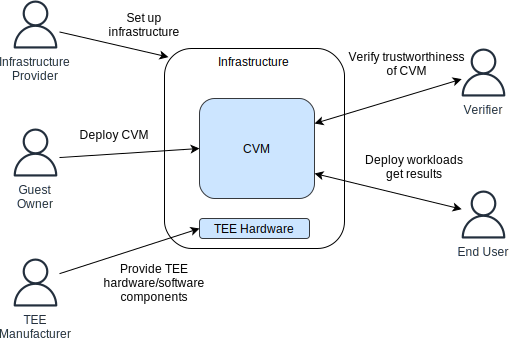
\includegraphics[width=.9\columnwidth]{figures/system-model.drawio.pdf}
    \caption{System Model and logical actors involved in the deployment of a
    \ac{CVM}.}
    \label{fig:system-model}
\end{figure}
\fi

In our system model, a guest owner deploys a \ac{CVM} on an infrastructure where
potentially other software is running at the same time, such as other VMs
(confidential or not), monitoring software, etc. The infrastructure is managed
by an infrastructure provider, and should provide the hardware and software
primitives required to run the \ac{CVM} in a \ac{TEE}. Besides, a verifier
performs attestation to make sure that the \ac{CVM} was deployed and booted
correctly; We refer to the IETF RATS architecture for a more comprehensive
representation of the attestation infrastructure~\cite{ietfRats}. Furthermore,
an end user interacts with the \ac{CVM} to, e.g., deploy workloads and retrieve
results. In general, some interaction between such actors is required and trust
relationships between them may vary according to the use case. Besides, two or
more logical actors can, in practice, be impersonated by the same party: For
example, when running a \ac{CVM} on a local machine, all actors may be played by
the owner of that machine. When deploying a \ac{CVM} in the cloud, however, all
actors are likely unique. We will discuss this scenario in more detail in
\cref{sec:scenario}.

In this paper, we follow the standard threat model of \acp{TEE}: All software
running outside of the \ac{CVM} is potentially malicious, including the
VMM/hypervisor, other VMs, etc. Note that this is true even when the guest owner
and the infrastructure provider are the same party or trust each other, since
the software running on the infrastructure might be compromised by remote
attackers. Instead, the \ac{TEE} manufacturer and any software and hardware
components provided by them are assumed to be secure. The \ac{TEE} threat model
mainly focuses on confidentiality and integrity but leaves out availability.
Additionally, side channels and physical attacks are also out of scope.

\subsection{The Importance of Remote Attestation}

\iffalse
\begin{figure}[t]
  \centering
    \includegraphics[width=.7\columnwidth]{figures/report.drawio.pdf}
  \caption{Representation of a generic \ac{TEE} attestation report. Information
  about the platform TCB and a digital signature bind the \ac{TEE} instance to a
  specific node. A \emph{launch measurement} along with a policy give
  information on the code and data running on the \ac{TEE} instance. User data
  may bind a credential owned by the \ac{TEE} instance to the attestation
  report. Finally, the report may contain other \ac{TEE}-specific fields that
  provide additional claims.}
  \label{fig:report}
\end{figure}
\fi

\begin{figure}[t]
  \centering
    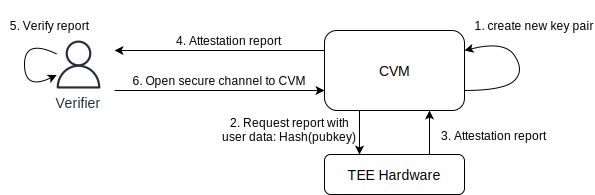
\includegraphics[width=.99\columnwidth]{figures/attestation-flow.drawio.pdf}
  \caption{High-level attestation flow.}
  \label{fig:attestation-flow}
\end{figure}

When it comes to \acp{TEE}, remote attestation is an essential step to gain
confidence in the deployed \ac{CVM}, making sure that, after boot:
\begin{inparaenum}
    \item the \ac{CVM} is running in a genuine and up-to-date \ac{TEE}, and
    \item the \ac{CVM} is in an expected and good state, i.e., only trustworthy
      and measured software has been loaded.
\end{inparaenum}
Moreover, attestation is often used to bind the identity of the \ac{CVM} to a
cryptographic credential, later used to establish a secure channel for
provisioning secrets and deploying workloads, e.g., via SSH or TLS connections.
Figure~\ref{fig:attestation-flow} shows how this is usually achieved.

After generating an ephemeral key pair (step 1), the \ac{CVM} embeds some
information about the credential in the attestation report requested from the
TEE hardware (step 2). This could include, e.g., a hash of the public ephemeral
key as well as a nonce provided by the verifier for freshness (not shown). The
signed attestation report returned by the TEE hardware (step 3) then includes
this data along with information about the TEE hardware and measurements of
software deployed in the TEE. After receiving and verifying the report (steps 4
\& 5), the verifier can now be certain that the key is \emph{owned} by a
\ac{CVM} with the specific hardware and software configuration matching the
attestation report.

When attestation fails, this binding becomes compromised, and the verifier (or
other entities) cannot be sure that they are communicating with a legitimate
\ac{CVM}. The problem is exacerbated by the complexity of \ac{CVM} attestation
that might lead to some components being accidentally skipped during
verification. In the next sections, we describe all steps of \ac{CVM}
attestation and show what might happen when some of these steps are missed.

\subsection{Attestation Levels}
\label{section:att-levels}

\begin{figure}[t]
    \centering
      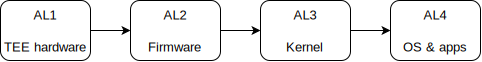
\includegraphics[width=.9\columnwidth]{figures/levels-v2.drawio.pdf}
    \caption{Hierarchy of attestation levels for \acp{CVM}.}
    \label{fig:attestation-levels}
\end{figure}

Attesting a \ac{CVM} is not an easy task since we need to ensure that every part
of the boot process is measured and can be verified. This section identifies
five stages of attestation of a \ac{CVM}, called \emph{Attestation Levels (ALs)}.
These levels are incremental, meaning that the guarantees provided at a certain
level build upon the levels below. A visual representation of such levels is
provided in \cref{fig:attestation-levels}.

\noindent\textbf{\emph{AL0: No attestation.}}
%
This is the baseline level where no attestation is done. As a result, the
verifier cannot make any claims on the state of the \ac{CVM} and the threat
model is the same as for a regular VM execution environment.

\noindent\textbf{\emph{AL1: Attested \ac{TEE} isolation.}}
%
In this level, the verifier has access to the ``raw'' attestation report signed
by the \ac{TEE} manufacturer, and is able to independently verify its integrity
and authenticity. This typically involves the verification of the report's
signature and certificate chain, which goes up to a root certificate that is
self-signed by the \ac{TEE} manufacturer. Moreover, the report also contains
some information about the platform's \ac{TCB} (e.g., CPU model, microcode
version, etc.), and freshness information provided by the verifier. This allows
the verifier to attest that the \ac{CVM} is indeed running in a genuine and
up-to-date \ac{TEE}, which reduces the threat surface significantly as the host
firmware, OS, and virtualization layer can now be excluded from the TCB. The
verifier can also be sure now that software running outside of the CVM cannot
directly access data stored inside of it. However, threats specific to the CVM
technology used, e.g., side channel leakage, or to the software running inside
the \ac{CVM} remain.   

\noindent\textbf{\emph{AL2: Measured firmware.}}
%
As mentioned above, remote attestation is used to establish a secure channel
into the \ac{CVM}, but AL1 does not give any information about what software is
running at the other end of that channel. A first step to alleviate this
situation is verify the \emph{launch measurement} contained in the attestation
report, which reflects the memory layout of the \ac{CVM} at boot time including
the firmware, page metadata and CPU register state. To obtain evidence for the
correct deployment of the firmware, the verifier needs to validate the launch
measurement against a trusted reference value. That measurement in itself does
not tell anything about the code and data running in the \ac{CVM}, hence it is
important that the firmware's source code is available and can be reproducibly
built.  After a successful verification, it can be ruled out that the trusted
firmware has been replaced by a malicious one.

\noindent\textbf{\emph{AL3: Measured Kernel.}}
%
To rule out compromise of later boot stages, the verifier needs to validate the
entire boot chain that starts from the firmware and goes up to the kernel,
(optionally) through a bootloader. This also includes the initial RAM disk and
kernel command-line parameters. By default, these components are not measured by
the \ac{TEE} and thus not part of the launch measurement. However, there are
several ways to make this attestation possible, some of which are discussed in
\cref{section:att-examples}.

\noindent\textbf{\emph{AL4: Fully measured boot.}}
%
The verification of the measurements done at AL3 stops at \emph{early
userspace}, i.e., right before the root filesystem is mounted to the \ac{CVM}.
At the very least, the root filesystem of the \ac{CVM} containing OS and
application data should be integrity protected, to prevent loading a malicious
version. In case it contains secrets, it should also be encrypted. The challenge
in this step is to securely provision keys to the \ac{CVM} only after a
successful AL3 attestation, to prevent leaking the keys to a compromised
\ac{CVM}. Again, possible implementation strategies are provided in
\cref{section:att-examples}.

After a successful AL4 attestation, the verifier has confidence that the desired
system and application software has been deployed correctly in the \ac{CVM}. At
this point, the threat model is similar to running the guest system on a trusted
dedicated server and run-time security of the \ac{CVM} is under the guest
owner's purview. In particular, the deployed software may employ security
policies to sanitize untrusted inputs or prevent the loading of additional,
untrusted software. Moreover, further attestation steps may be initiated by the
guest owner, e.g., run-time attestation of application control-flow integrity,
or attesting the authenticity of attached secure I/O devices.

\subsection{Attestation Strategies}
\label{section:att-examples}

Typically, support for AL1 and AL2 attestation is provided by all \ac{TEE}
manufacturers, via a certificate chain and a public key infrastructure (for AL1)
and a a measurement of the initial memory layout of the \ac{CVM} (for AL2). In
both cases, it is often sufficient to verify the attestation report that can be
fetched by the \ac{CVM} and sent to the verifier. To reach ALs 3 and 4, instead,
additional steps are needed. Below, we discuss possible approaches.

\noindent\textbf{\emph{AL3.}}
%
A simple strategy to make this attestation possible leverages Direct Linux Boot
to bind kernel measurements to the firmware, in such a way that the launch
measurement in the attestation report also reflects the identity of kernel
components~\cite{kernelHashesOvmf}. This can be done by adding kernel
measurements as firmware variables, which will be loaded into secure memory at
boot and measured by the \ac{TEE}. Then, the firmware will load and pass control
to the kernel only if its measurements match with the expected ones stored as
variables, aborting otherwise. A more involved solution involves relying on a
\ac{vTPM} for measuring the \ac{CVM} boot chain. On AMD SEV-SNP, this
functionality can be exposed thanks to \acp{VMPL}~\cite{AmdSevAbi}, where the
\ac{vTPM} executes in a higher privilege level than the rest of the system. To
bind \ac{vTPM} quotes to \ac{TEE} attestation reports, the digest of the
\ac{vTPM} endorsement key is added as user data in the \ac{TEE}
report~\cite{narayanan2023svsm}. The verifier, then, has to check both the
report and the quote to verify the trustworthiness of the \ac{CVM}. On Intel
\ac{TDX}, instead, a \ac{vTPM} can be exposed from a separate trust
domain~\cite{intelTdxvTPM}. Additionally, Intel \ac{TDX} also provides four
\acp{RTMR} whose value is reflected in the attestation
report~\cite{intelTdxModule}. These registers are analogous to a \ac{TPM}'s
PCRs, and can be similarly leveraged by a TDX-aware firmware to measure boot
components.

\noindent\textbf{\emph{AL4.}}
%
To ensure the integrity of the root filesystem, a common approach is to extend
the \ac{vTPM} measurements up to the user space with Linux
\ac{IMA}~\cite{sailer2004ima}. \ac{IMA} is a kernel subsystem responsible for
measuring all binaries that are loaded at runtime, and it supports remote
attestation. Measurements are stored in a measurement file which itself is
integrity-protected by a measurement stored in the TPM, to prevent tampering
from a privileged adversary. When adopting \ac{IMA}, it is important to be aware
that runtime measurements may be susceptible to time-of-check-time-of-use
attacks~\cite{bohling2020imatoctou}, and that there exist so-called
\emph{measurement gaps}, i.e., some components are not measured.

Another approach relies on protecting the integrity of the whole filesystem at
rest. 
%The Linux Kernel offers a functionality called \emph{device mapper}, for
%mapping physical block devices to higher-level virtual block devices. This
%mapping allows checking and/or modifying data in transit to and from the
%physical block devices, and can be leveraged to guarantee confidentiality,
%integrity and authenticity of a filesystem. 
To this extent, a popular software solution is \dmverity~\cite{dmVerity}, which
provides integrity protection by verifying the data blocks in a filesystem
against pre-computed hash values, stored as a Merkle tree on a separate disk.
The root of the tree (called root hash), guarantees integrity of the whole
filesystem, and must protected from tampering. In our attestation flow, the root
hash can be provided as a kernel parameter such that its integrity can be
verified with a AL3 attestation. Filesystems using \dmverity{} are mounted as
read-only; To enable both read and write, \dmintegrity{}~\cite{dmIntegrity} can
be leveraged instead to (re-)compute HMAC tags for each sector of the block
device. In this case, however, a key should be separately provisioned to the
kernel during early userspace. In our \ac{CVM} scenario, this means that
attestation should be performed during boot. Finally, \dmintegrity{} can be
combined with \dmcrypt{}~\cite{dmCrypt} to additionally provide encryption.

\subsection{Partial Attestation}
\label{section:partial-attestation}

\begin{figure}[t]
  \centering
    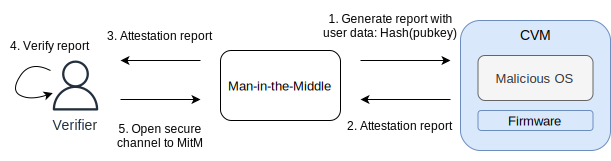
\includegraphics[width=\columnwidth]{figures/partial-attestation.drawio.pdf}
  \caption{Possible Man-in-the-Middle attack with an unverified guest OS.}
  \label{fig:partial-attestation}
\end{figure}


It should now be clear that attesting a \ac{CVM} is not a trivial task. Unlike
process-based \acp{TEE} such as Intel SGX, verifying the \ac{TEE} attestation
report alone is necessary but \emph{not sufficient} to cover the whole boot
process of the confidential workload. Failing to properly verify one or more
boot stages might cause some attacks to go undetected, such as injecting
malicious code or backdoors that would compromise the integrity and
confidentiality of the \ac{CVM}. These kind of attacks can be either local
(e.g., a compromised hypervisor tampering with the root filesystem) or remote
(e.g., a malicious kernel image downloaded from an untrusted
registry). Therefore, partial attestations might give a false sense of security
to guest owners and end users, who expect that their code and data is protected
when, in reality, this might not be true.

To showcase the severity of partial attestations, we consider the scenario where
the verifier only attests the \ac{CVM} up to AL2. Here, a \ac{MitM}
attack is possible if the \ac{CVM} loads a malicious OS
(\cref{fig:partial-attestation}): As the \ac{CVM} can produce attestation
reports with arbitrary user data, a \ac{MitM} that controls the \ac{CVM} OS can
bind the report with a credential owned by the \ac{MitM} (step 1). The verifier,
when receiving the attestation report (step 3), can successfully verify that the
report comes from a genuine \ac{CVM} with the expected firmware (step 4), but
cannot make any claims on the running OS. Failing to recognize this issue might
cause the verifier to bind the \ac{CVM} identity to the credential owned by the
\ac{MitM}, leading to the verifier possibly opening a channel with the \ac{MitM}
and leak secrets (step 5). What is worse, the \ac{MitM} does not even need to
run in a \ac{CVM}, meaning that all data will be processed in clear. Therefore,
although the verifier has performed a successful AL2 attestation, in
practice the security guarantees obtained are basically the same as without
attestation.

\section{CVM Attestation in Public Clouds}
\label{sec:scenario}

Above, we have discussed the different attestation levels a verifier can achieve
when evaluating the authenticity and integrity of a deployed \ac{CVM}.  However,
who exactly plays the role of verifier depends greatly on the application
scenario and the trust relations between the involved parties.  In this work, we
focus on a scenario where a tenant wants to deploy a \ac{CVM} as guest owner on
a cloud platform, acting as the verifier in the attestation process. Afterwards,
attestation results may also be exposed to end users as
well~\cite{galanou2023revelio}. While different tenants may have different trust
relations with a given \ac{CSP} and lower attestation levels may suffice for
them in practice, we assume here that the tenant wants to reduce the required
trust in the infrastructure provider as much as possible and achieve a high
level of trustworthiness for the \ac{CVM} solution via attestation. 

Here, the measurement reports used during attestation should ideally be
verifiable independently of the \ac{CSP}. In particular, attestation reports
produced by the \ac{TEE} hardware need to be available to the verifier. In
addition, the verifier needs to be able to identify trusted software deployed in
the \ac{TEE}, i.e., they need to know the corresponding reference measurements
for the firmware, kernel, user applications, etc. A \ac{CSP} may provide these
reference values so that the authenticity of the deployed software can be
established. However, this results in a notion of verifiability that still
relies on trust in the \ac{CSP} and in the security of the deployed software. In
principle, a trusted third party such as Intel Trust
Authority~\cite{intelTrustAuthority} could certify the security of that software
and publish the corresponding reference values, but that just shifts the
required trust to a different entity.

A stronger \emph{verifiability without trust} entails that the verifier can
inspect the source code of software deployed in the \ac{TEE} and obtain the
reference measurements via a reproducible build process. Having access to the
source code allows the verifier to conduct their own security analysis of the
code and judge its trustworthiness. Of course, if the code is publicly
available, this review can also be performed by the open source community, but
this would again introduce required trust into the picture.

Overall, for our cloud \ac{CVM} scenario, the tenant wants to achieve
verifiability without trust for as high an attestation level as possible. Even
if a high \emph{nominal} AL can be achieved with the help of the \ac{CSP}, still
being
forced to trust the \ac{CSP} blindly for the measurement values and deployed
software reduces the trustworthiness. We introduce the term \emph{trustworthy
AL} to denote the maximum, effective attestation level the tenant can achieve as
a verifier without trust into the public cloud provider.
%\input{chapters/sev-snp.tex}
\section{Exploring the Cloud Landscape}
\label{section:cloud}

\newcommand{\pie}[1]{%
\begin{tikzpicture}
 \draw (0,0) circle (1ex);\fill (1ex,0) arc (0:#1:1ex) -- (0,0) -- cycle;
\end{tikzpicture}%
}

\newcommand{\revpie}{%
\begin{tikzpicture}
 \draw (0,0) circle (1ex);\fill (0,1ex) arc (90:270:1ex) -- (0,0) -- cycle;
\end{tikzpicture}%
}

\newcommand{\tableYes}{\pie{360}}
\newcommand{\tableNo}{\pie{0}}
\newcommand{\tablePartial}{\revpie}

\begin{table}[!t]
    \renewcommand{\arraystretch}{1.35}
    \newcolumntype{L}{>{\raggedleft\arraybackslash}X}
    \newcolumntype{C}{>{\centering\arraybackslash}X}
    \newcolumntype{R}{>{\raggedright\arraybackslash}X}
    \centering

    \begin{tabularx}{.9\linewidth}{l C C C}
        \toprule
                                           & AWS           & Azure         & GCP           \\
        \hline                                                              
        TEE                                & \tableYes     & \tablePartial & \tableYes     \\
        Firmware                           & \tableYes     & \tablePartial & \tablePartial \\
        Kernel                             & \tablePartial & \tablePartial & \tablePartial \\
        Root FS                            & \tablePartial & \tablePartial & \tablePartial \\
        \hline                                                              
        \textbf{Nominal AL}                & \textbf{4}    & \textbf{4}    & \textbf{4}    \\
        \textbf{Trustworthy AL}            & \textbf{2}    & \textbf{0}    & \textbf{1}    \\
        \bottomrule
    \end{tabularx}

        \vspace{0.2cm}
        {\raggedright \tableYes\xspace= Verifiable w/o trust; \tablePartial\xspace= Verifiable w/ trust; \tableNo\xspace= Not verifiable \par}
        \vspace{0.2cm}
        \caption{AMD \sevsnp{} offerings on \ac{AWS}, Azure and \ac{GCP}. This
          table reflects attestation levels described in
          \cref{section:att-levels} and verifiability with or
          without trust, resulting in the maximum nominal AL (with trust in the
          \ac{CSP}) and trustworthy AL (without trust). Results dated \clouddate.}
        \label{tbl:cloud-landscape}
        %\vspace{-5mm}
\end{table}
%
  


We investigated current \ac{CC} offerings on public clouds, focusing on
\sevsnp{} as the most widely available VM-based \ac{TEE}. Our evaluation is
solely based on commercial cloud features under general availability or public
preview. We found that only the three major \acp{CSP}, i.e., Microsoft Azure,
\ac{GCP} and \ac{AWS}, offer to deploy \sevsnp{} \acp{CVM} on demand. We looked
for VM-based confidential computing support in other \acp{CSP}, but they either
supported plain \sev{} or only offered single-tenant bare-metal servers with
\sevsnp{} hardware. While plain \sev{} does not provide integrity protection nor
flexible attestation capabilities, bare-metal servers come at much higher costs
and typically require a fixed monthly subscription. Instead, we were interested
in the multi-tenant scenario where customers can deploy \acp{CVM} on demand on a
shared infrastructure, with little to no control over the hypervisor.

As discussed in \cref{sec:scenario}, our evaluation tried to determine the level
of \emph{verifiability without trust} that can be achieved on such
\acp{CSP}. Besides, we also considered the model where the verifier (partially)
trusts the \ac{CSP} and relies on provided services and data, such as a custom
attestation report or a proprietary attestation service.

Results are shown in \cref{tbl:cloud-landscape} and based both on public
documentation and direct experiments. Regarding the former, all references in
\cref{eval:cloud-results}, except Github links, have been uploaded to the
Internet Archive\footnote{\url{https://www.archive.org}} to provide a stable
reference. Concerning the latter, our evaluation was made on \clouddate{}. Since
this is a snapshot of the current state and features of clouds, some of our
findings may not hold in the future. However, our evaluation framework is still
useful to evaluate future offers in the \ac{CVM} area.

\subsection{Results}
\label{eval:cloud-results}

In our experiments on \ac{AWS} and \ac{GCP}, we were able to fetch a raw
attestation report from the AMD \ac{SP} via the \sevguest{} device, allowing to
independently verify that the guest VM is indeed running in a up-to-date
\sevsnp{} \ac{TEE}. Azure \acp{CVM}, instead, only provide access to an
attestation report generated at boot time and stored in \ac{vTPM} non-volatile
memory. As this report does not contain any freshness information chosen by the
verifier, the latter cannot distinguish a legitimate attestation report from a
replay attack and must rely on the \ac{CSP} to attest that the VM is indeed
using \sevsnp. We tried to boot an \snp{}-aware kernel built from the AMDSEV
repository~\cite{amdsevGithub}, yet we still could not access the AMD \ac{SP}.

Regarding AL2, only \ac{AWS} offers an open source firmware that can be
reproducibly built~\cite{awsUefi}. We successfully checked that the attestation
report indeed reflects the correct measurement. Instead, Azure and \ac{GCP}
guests boot a proprietary firmware whose code cannot be audited. To the best of
our knowledge, firmware reference measurements are also not provided, meaning
that the verifier cannot even compare the measurement in the attestation report
against the expected value. However, we observed that both Azure and \ac{GCP}
have a secure boot option that prevents \acp{CVM} from booting if the firmware
is corrupted~\cite{azureDocsSecureBoot,googleDocsSecureBoot}, though we could
obviously not experimentally verify this claim. Yet, tenants that are willing to
trust their \ac{CSP} can be confident that a running firmware was not tampered
with by an outsider attacker.

All \acp{CSP} allow extending the measurements up to the kernel via a \ac{vTPM}.
However, on \ac{AWS}~\cite{awsGithubvTPM} and \ac{GCP}~\cite{googleDocsvTPM} the
\ac{vTPM} is implemented in the hypervisor, greatly increasing the \ac{TCB}.
Azure, instead, exposes a \ac{vTPM} from within the \ac{CVM}
firmware~\cite{azureDocsvTPM} which, as mentioned before, cannot be reviewed.
Thus, no \ac{CSP} currently supports trustworthy attestation of kernel
components.

After kernel verification, the chain of measurements can be extended to the root
filesystem via different approaches (\cref{section:att-examples}).  Hence, AL4
is a natural extension of AL3, provided that the \ac{CSP} allows for the
customization or upload of VM images by the guest owner. We experimentally
verified that the former is indeed possible by installing a custom bootloader
and kernel, as well as changing kernel command-line parameters, e.g., to enable
Linux \ac{IMA}. Uploading images seems also feasible according to public
documentation~\cite{awsDocsCustomImage,azureDocsCustomImage,googleDocsCustomImage},
but we did not verify this. Still, for trustworthy attestation, the integrity of
the root filesystem ultimately relies on the integrity of the boot chain up to
the kernel: If the latter cannot be verified independently of the \ac{CSP},
neither can the former.

In summary, all \acp{CSP} provide the infrastructure to perform a full
attestation (\emph{nominal AL4}), but they rely on either proprietary software
or components outside the \ac{TEE} TCB, or both. On Azure, a verifier can obtain
an attestation report but cannot verify its freshness, hence replay attacks are
possible and the \ac{CSP} must be trusted for all attestation levels
(\emph{trustworthy AL0}). On \ac{GCP}, one can fetch dynamic reports, but the
firmware cannot be independently verified (\emph{trustworthy AL1}). Only
\ac{AWS} allows to attest an auditable firmware, yet extending the chain of
measurements to later boot stages uses a hypervisor-based \ac{vTPM} outside the
\ac{TEE} (\emph{trustworthy AL2}).

\subsection{Discussion}

We showed that guest owners still require a significant amount of trust
in the \acp{CSP} when using \ac{CVM} solutions in the cloud. This goes against
the classic \ac{TEE} threat model, where the infrastructure is considered
untrusted. There are two reasons for this:
%
\begin{inparaenum}
    \item \ac{CSP} code is running inside the \ac{TEE} boundary, with no
    possibility for review by the remote verifier, and
    \item the attestation process involves \ac{CSP}-managed components.
\end{inparaenum}
%
While running \ac{CSP} code in the \ac{CVM} is sometimes necessary (e.g., to
configure network interfaces, mount devices, etc.), it is certainly possible to
increase transparency towards the verifier, as demonstrated by \ac{AWS}'
reviewable firmware. The second problem is mostly caused by a lack of
customization options offered by \acp{CSP}. This is somewhat understandable
since most cloud customers are looking for ease of use and ``one-click
compliance'', where they are willing to trust the \ac{CSP} to perform security
checks in their place. For advanced users, however, more customizability is
desirable.

%There is also a fundamental challenge with VM-based \acp{TEE}, which lies on the
%management of measurements. As we have seen throughout the paper, there are
%multiple software components that need to be measured, which may come from
%different stakeholders. Besides, some of them undergo frequent updates that
%further increase the number of "golden measurements" to manage. Here, it may be
%desirable to rely on a trusted third party that keeps a database of acceptable
%measurements and associated metadata.

Our evaluation did not focus on userspace software that runs after booting the
root filesystem, such as \texttt{cloud-init}~\cite{cloudInit} or
\ac{CSP}-managed software like Azure Linux VM Agent~\cite{azureDocsLinuxAgent}.
These agents take care of VM configuration and can execute privileged commands,
like installing packages or updating the trusted SSH identities. Any such
operation, if compromised, can thwart the security guarantees of
\acp{CVM}. Hence, it is equally important to implement hardening measures in the
root filesystem to, e.g., check \texttt{cloud-init} configuration files before
executing them or disable unnecessary software.

Lately, several companies like Anjuna~\cite{anjuna}, Edgeless
Systems~\cite{edgelessSystems}, and Enclaive~\cite{enclaive} have started
offering their own confidential computing solutions to customers, providing
fully-managed confidential workloads in form of containers, virtual machines, or
both, and supporting deployments on popular \acp{CSP}. Attestation of workloads
is managed by a dedicated attestation service (which can also run within a
\ac{TEE}) and is therefore transparent to the customer, who only receives a
report indicating whether or not their deployment is verified. Such solutions
can largely improve user experience and ease the adoption of confidential
computing. However, when it comes to cloud deployments, they still depend on the
\acp{CSP} and the confidential computing features offered by them.  Therefore,
besides adding another third party to the trust model, such solutions cannot
increase the \emph{trustworthy AL} shown in \cref{tbl:cloud-landscape}.
Analogously, the same applies to third-party attestation services such as Intel
Trust Authority~\cite{intelTrustAuthority}.

A possible solution to the trust problem could leverage the live migration
feature of \acp{TEE} to initialize a \ac{CVM} locally and then migrate its state
to a remote host, where it continues its execution. Live migration is performed
over a secure channel established between the \ac{TEE} modules in both hosts,
preserving the confidentiality and integrity of the \ac{CVM}. Since the \ac{CVM}
is initialized on a local platform, the guest owner has full control over its
boot process and could therefore implement a full \emph{AL4} attestation
strategy. Live \ac{CVM} migration is supported by AMD \sevsnp{} and Intel
\ac{TDX}~\cite{AmdSevSnpWhitepaper,intelTdxMigration}. However, apart from some
technical and organizational challenges (e.g., the guest owner needs proper
\ac{TEE} hardware to initialize the \ac{CVM}), this workflow is currently not
supported by any \ac{CSP} and thus we did not explore it further.

Finally, we note that CC is still a relatively new technology and support for
recent \acp{TEE} such as \sevsnp{} in the cloud has not yet reached maturity. On
the evaluated \acp{CSP}, \acp{CVM} are currently available in selected regions
only and, on \ac{GCP}, support is in public preview. Despite existing
limitations, we see many efforts from \acp{CSP} to improve their offering,
driven in part by the open source community and standardization bodies. For
example, Google has recently open-sourced an unofficial tool to verify the
firmware of \acp{CVM} running on \ac{GCP}~\cite{gceTcbVerifier}, which
potentially allows reaching a trustworthy \emph{AL2}.

%\input{chapters/discussion.tex}
\section{Conclusions}
%
Being marketed as a solution that allows for the ``removal
of even the cloud provider from the Trusted Computing
Base''~\cite{confcon2022marketing}, which has
caught the attention of customers who need an additional layer of protection for
intellectual property, sensitive data, or for regulatory compliance in data
protection, confidential computing is becoming a mainstream technology for
cloud-based services.
% When it comes to cloud deployments, TEEs can also be leveraged to comply
% with regulations such as GDPR.
%
However, our research shows that, today, the promised security guarantees are
far from reality as cloud providers still play a crucial role in the deployment
and management of confidential workloads, especially regarding the latest trend
with confidential virtual machines. Yet, customers that are willing to trust the
CSPs can still benefit from current offerings as a defense-in-depth mechanism
for strong hardware-rooted isolation from other tenants and the hypervisor.
%
We also notice a joint effort between cloud providers and organizations such as
the Confidential Computing Consortium and the IETF, as well as the open source
community, to enhance current confidential computing solutions. Here,
researchers can play an important role and nudge actors towards more principled
security.



\ifdefined\CAMERAREADY
\section*{Acknowledgements}
This research is partially funded by the Research Fund KU Leuven, by the
Cybersecurity Research Program Flanders, and by the CyberExcellence programme of
the Walloon Region, Belgium (convention no. 2110186). This research has received funding under EU H2020
MSCA-ITN action 5GhOSTS (GA no. 814035). We especially thank Fritz
Alder and Thomas Nyman for their valuable feedback and insights.
\fi

\balance
%\IEEEtriggeratref{24}
%%
%% The next two lines define the bibliography style to be used, and
%% the bibliography file.
\bibliographystyle{IEEEtranS}
\bibliography{bibliography}

%%
%% If your work has an appendix, this is the place to put it.
% \appendix


\end{document}
\endinput
%%
%% End of file `sample-sigconf.tex'.
